% This is my HW 4 solution set.

\documentclass[12pt, leqno]{article}
\usepackage{amsfonts, amsmath, amssymb}
\usepackage{fancyhdr}
\usepackage{hyperref}
\usepackage{graphicx}
\newcounter{qcounter}
\usepackage[lofdepth,lotdepth]{subfig}
\usepackage[maxfloats=40]{morefloats}
\usepackage{float}
\usepackage{}
\usepackage[english]{babel}
\usepackage{tabularx}
\providecommand{\abs}[1]{\lvert#1\rvert}
\providecommand{\norm}[1]{\lVert#1\rVert}
\newcommand{\macheps}{\epsilon_{\mbox{\scriptsize mach}}}
\usepackage[ampersand]{easylist}
\makeatletter
\newcommand{\distas}[1]{\mathbin{\overset{#1}{\kern\z@\sim}}}%
\newsavebox{\mybox}\newsavebox{\mysim}
\newcommand{\distras}[1]{%
  \savebox{\mybox}{\hbox{\kern3pt$\scriptstyle#1$\kern3pt}}%
  \savebox{\mysim}{\hbox{$\sim$}}%
  \mathbin{\overset{#1}{\kern\z@\resizebox{\wd\mybox}{\ht\mysim}{$\sim$}}}%
}
\makeatother

\begin{document}
\pagestyle{fancy}
\lhead{Syed Rahman}
\rhead{STA6866}

\begin{center}
{\large {\bf Homework 4}} \\
\end{center}
\paragraph{1.}
We assume that $\lambda_1$ and $\lambda_2$ have prior distribution
$gamma(a,b)$. Using the fact that the first quartile is 10 months and
the third quartile is 49 months and that $P(X>t) = b/(b+t)^a$ we solve for the following system of
equations to find the parameters $a$ and $b$:
\begin{align}
b/(b+10)^a &= 0.75 \\
b/(b+49)^a &= 0.25 
\end{align}

Using the package $nleqslv$ and initial values of $a = 2$ and $b =
0.5$ and a tolerance of $0.0001$ we get the solutions $a = 33.02833$ 
and $b = 1143.09157$.

\paragraph{2.}
We run a gibbs sampler to estimate the distribution of $\lambda_1$ and
$\lambda_2$. The density plots are included in Figures \ref{l1} and
\ref{l2}. We also estimate ${P(\lambda_1>\lambda_2)} = P(1/\lambda_1<1/\lambda_2)$ and we
do this using 
\[ \frac{1}{n} \sum_{i=1}^n I[\hat{\lambda}_1^i>\hat{\lambda}_2^i] =
0.19092
\]
This gives evidence that $E[X_2] = 1/ \lambda_2$ is most likely
greater than $E[X_1]$.

\begin{figure}
\centering
\subfloat[]
  {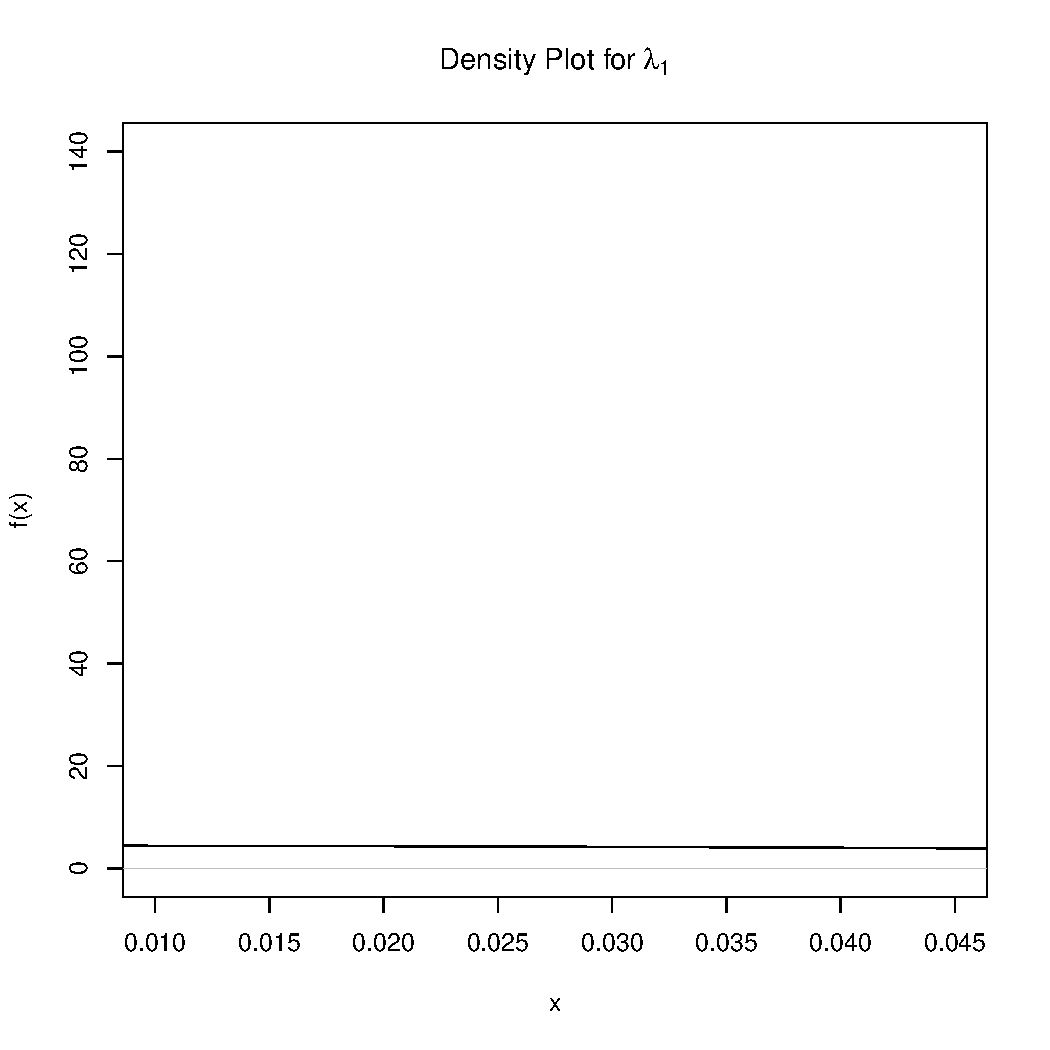
\includegraphics[scale = 0.45]{lambda1.pdf}
\label{l1}}
\centering
\qquad
\centering
\subfloat[]
  {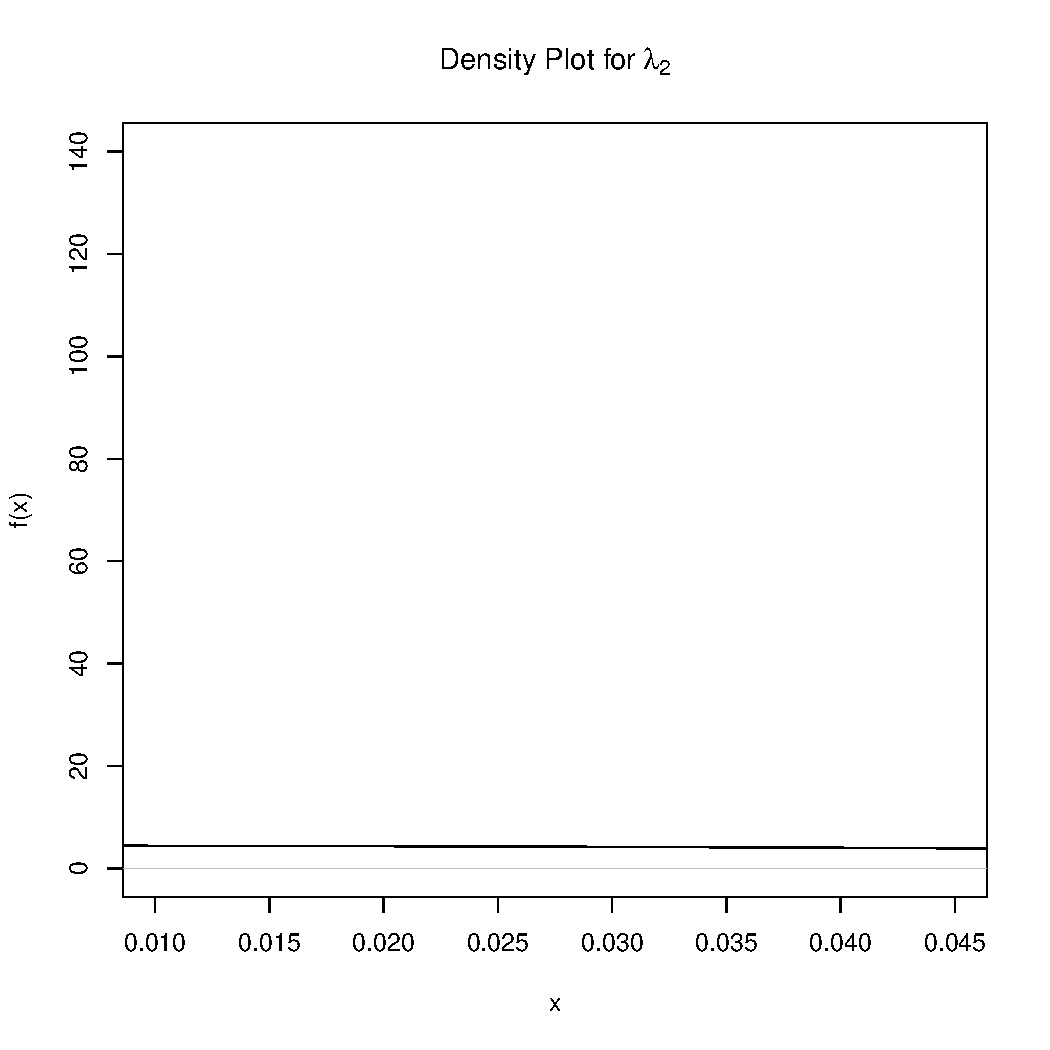
\includegraphics[scale = 0.45]{lambda2.pdf}
\label{l2}}
\caption{Density plot for $\lambda_1$ and $\lambda_2$}
\end{figure}

\paragraph{3.}

The posterior densities of $exp(-36 \lambda_j)$ for $j=1,2$ calculated by
multiplying the $\hat{\lambda}_j$'s by $-36$ and taking exponentials. The
densities are presented
in Figures \ref{el1} and \ref{el2}. 

\begin{figure}
\centering
\subfloat[]
  {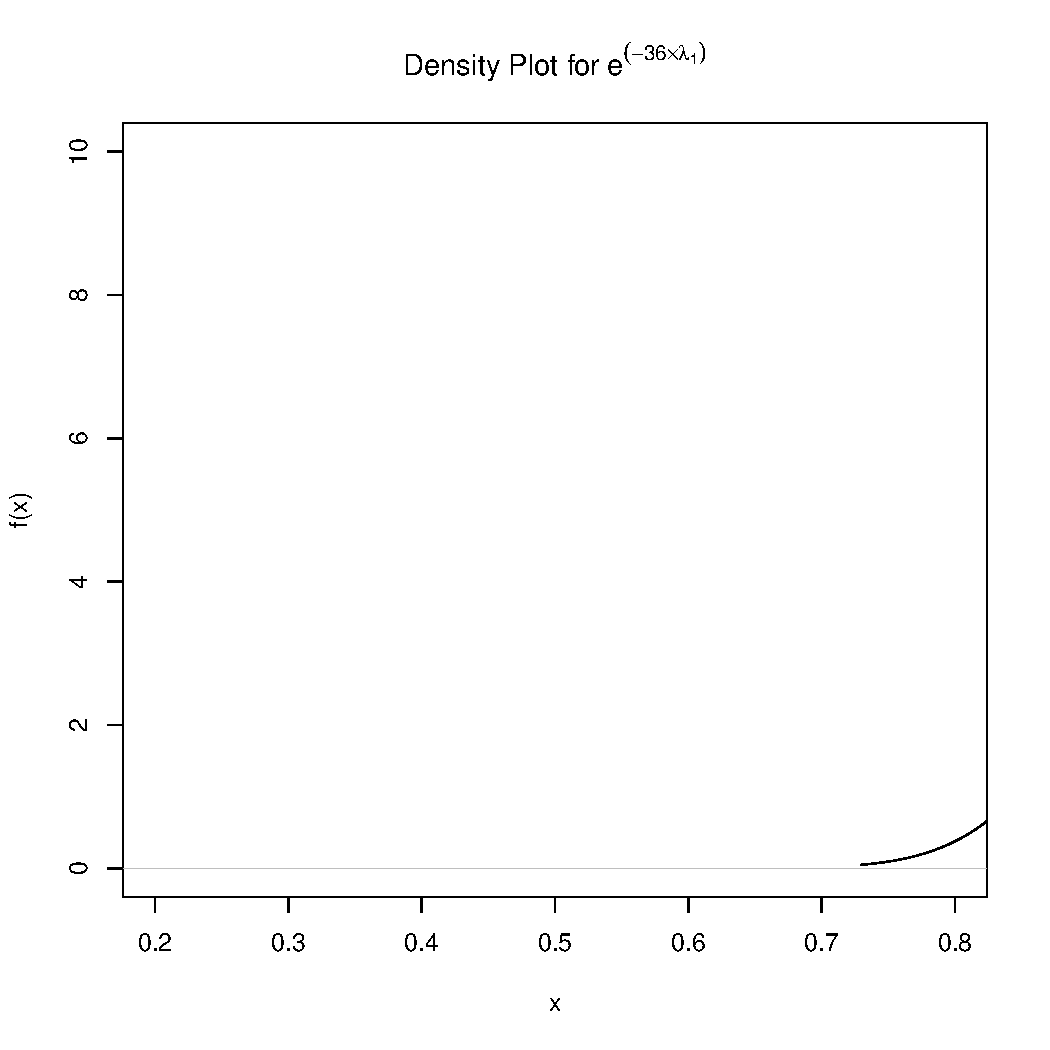
\includegraphics[scale = 0.45]{explambda1.pdf}
\label{el1}}
\centering
\qquad
\centering
\subfloat[]
  {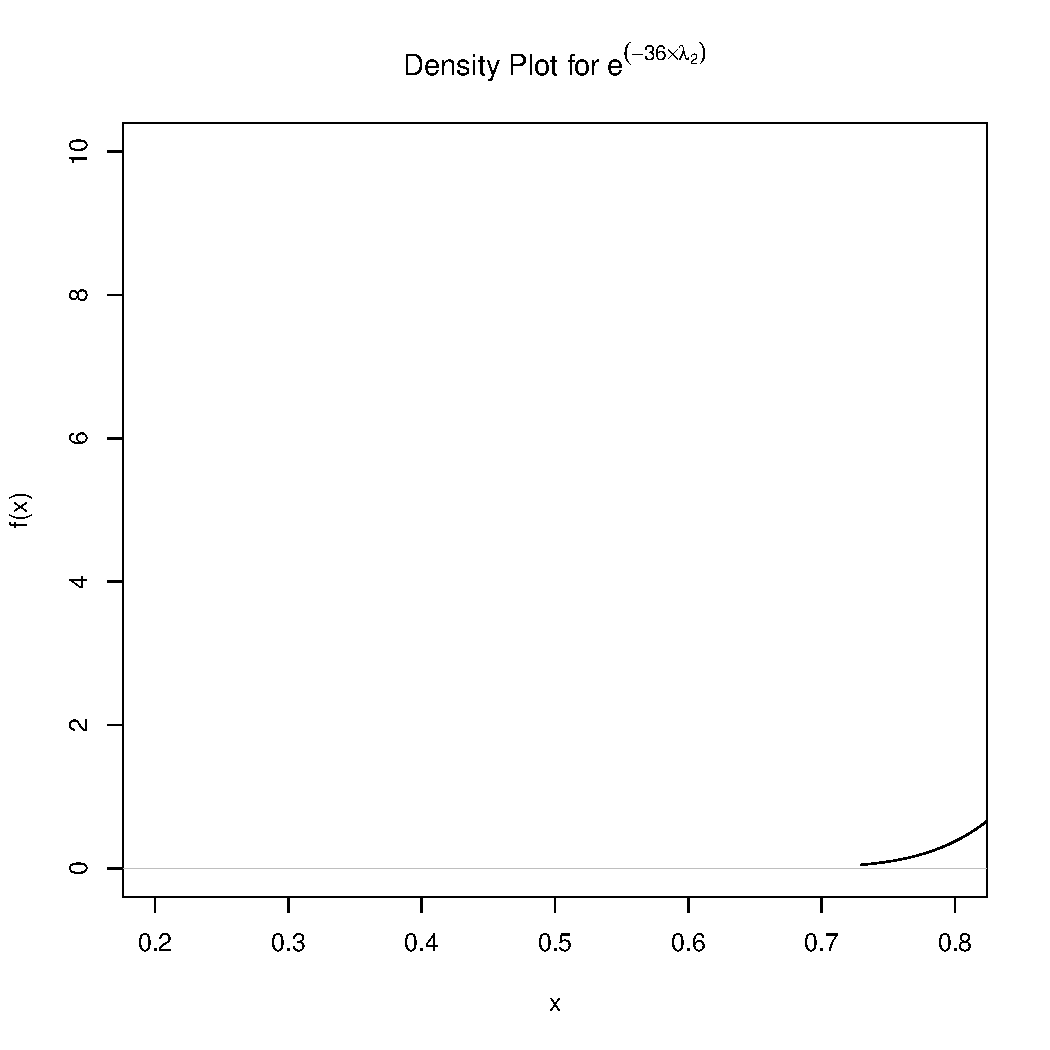
\includegraphics[scale = 0.45]{explambda2.pdf}
\label{el2}}
\caption{Density plot for $exp(-36 \lambda_1)$ and $exp(-36 \lambda_2)$}
\end{figure}

\paragraph{4.}

To find the posterior density of a new patient under treatment $j$, we
add create a new vector with the interval equal to $(0, \infty)$ in
the code for the gibbs sampler. The densities for a new patient under each treatment are
presented in Figures \ref{ml1} and \ref{ml2} for treatments 1 and 2 respectively.

\begin{figure}
\centering
\subfloat[]
  {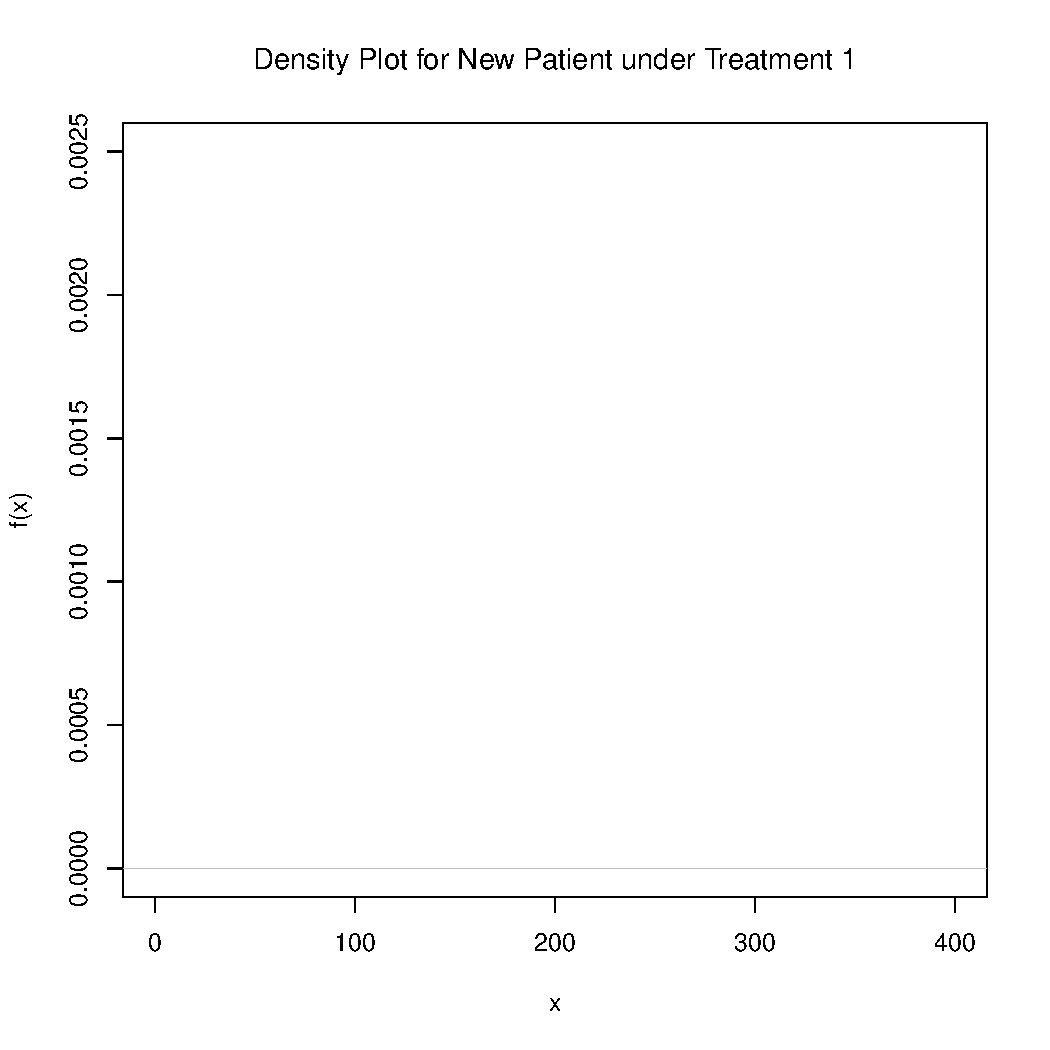
\includegraphics[scale = 0.45]{mlambda1.pdf}
\label{ml1}}
\centering
\qquad
\centering
\subfloat[]
  {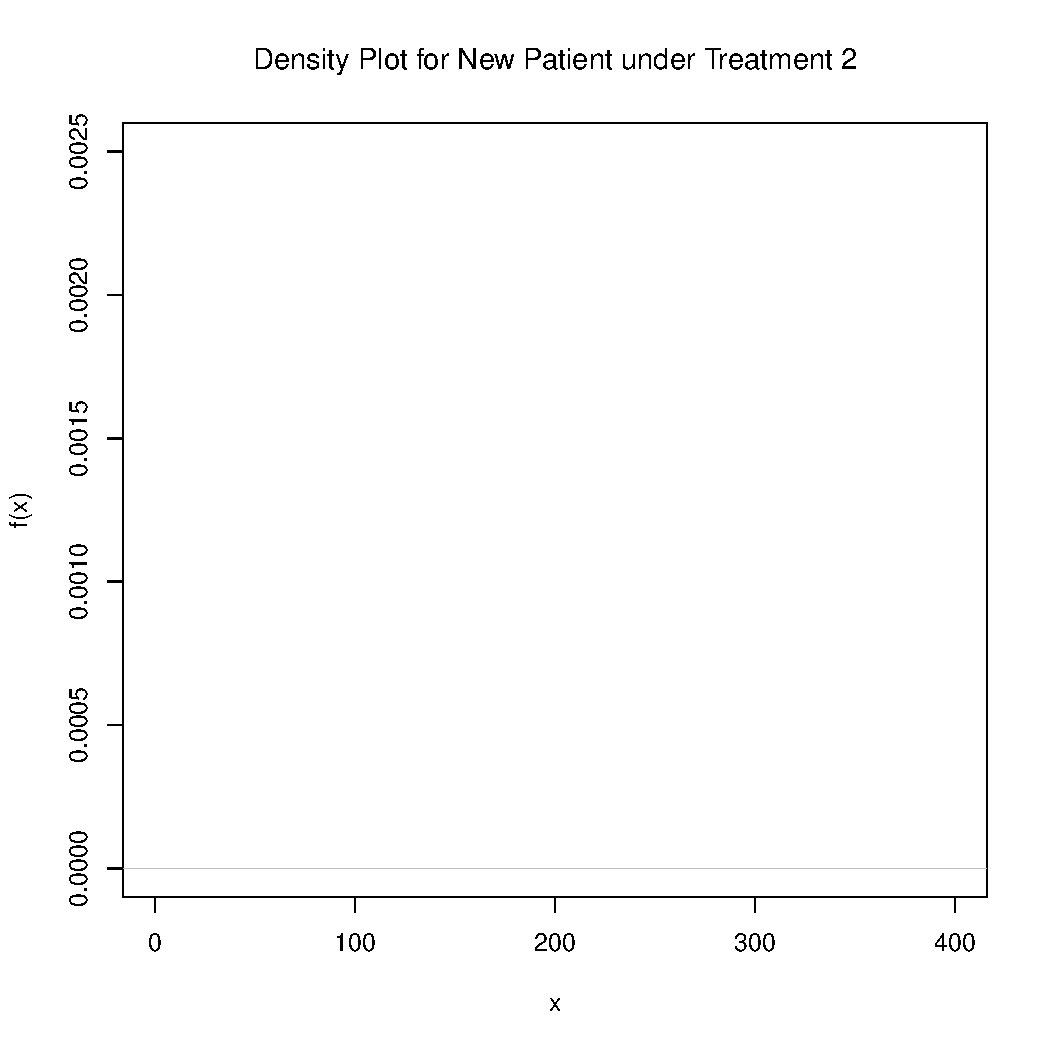
\includegraphics[scale = 0.45]{mlambda2.pdf}
\label{ml2}}
\caption{Density plot for the time to cosmetic deterioration for each treatment}
\end{figure}

\pagebreak

\paragraph{Appendix 1: R code and output}
\begin{verbatim}
model <- function(x) {
    F1 = (x[2]/(x[2]+10))^x[1] - 0.75
    F2 = (x[2]/(x[2]+49))^x[1] - 0.25
    c(F1 = F1, F2 = F2)
}
xstart <- c(2,0.5)
fstart <- model(xstart)
nleqslv(xstart, model, control=list(btol=.0001))

$x
[1]   33.02833 1143.09157

$fvec
[1]  2.361440e-09 -1.034709e-09

$termcd
[1] 1

$message
[1] "Function criterion near zero"

$scalex
[1] 1 1

$nfcnt
[1] 90

$njcnt
[1] 2

$iter
[1] 66

radio = read.table("breast-cancer-data-radiotherapy.txt",
header=TRUE,na.string = "---")
attach(radio)
U[is.na(U)]=Inf
lambda1 = 1
sum = sum(L)
a = 33.02833
b = 1143.09157
N = 46
nsim = 100000
lambda1 = rep(0,nsim)
u = rep(0,N)
x = rep(0,N)
unew = rep(0,1)
xnew1 = rep(0,nsim)
for (j in 1:nsim)
    {
        lambda1[j] = rgamma(n=1,a+N,(b+sum))
        lambdatemp= lambda1[j]
        low = pexp(L,rate = lambdatemp)
        up = pexp(U,rate = lambdatemp)
        u = runif(n=46,low,up)
        x = (-1/lambdatemp)*log(1-u)
        unew = runif(n=1,0,1)
        xnew1[j] = (-1/lambdatemp)*log(1-unew)
        sum = sum(x)
    }
radiochem = read.table("breast-cancer-data-radioandchemo.txt",
header=TRUE,na.string="---")
attach(radiochem)
U[is.na(U)]=Inf
lambdatemp = 1
sum = sum(L)
a = 33.02833
b = 1143.09157
N = 46
nsim = 100000
lambda2 = rep(0,nsim)
u = rep(0,N)
x = rep(0,N)
unew = rep(0,1)
xnew2 = rep(0,nsim)
for (j in 1:nsim)
    {
        lambda2[j] = rgamma(n=1,a+N,(b+sum))
        lambdatemp= lambda2[j]
        low = pexp(L,rate = lambdatemp)
        up = pexp(U,rate = lambdatemp)
        u = runif(n=46,low,up)
        x = (-1/lambdatemp)*log(1-u)
        unew = runif(n=1,0,1)
        xnew2[j] = (-1/lambdatemp)*log(1-unew)
        sum = sum(x)
    }
success = sum(lambda1>lambda2)
total = nsim
success/total

pdf("lambda1.pdf")
plot(density(lambda1),xlab = "x",ylab = "f(x)",
main = expression("Density Plot for" ~ lambda[1]),ylim=c(0,140),
xlim=c(0.01,0.045))
dev.off()
pdf("lambda2.pdf")
plot(density(lambda2),xlab = "x",ylab = "f(x)", 
main = expression("Density Plot for" ~lambda[2]),ylim=c(0,140),
xlim=c(0.01,0.045))
dev.off()
pdf("explambda1.pdf")
plot(density(exp(-lambda1*36)),xlab = "x",ylab = "f(x)",
main = expression("Density Plot for" ~ e^(-36%*%lambda[1])),
ylim=c(0,10),xlim=c(0.2,0.6))
dev.off()
pdf("explambda2.pdf")
plot(density(exp(-lambda2*36)),xlab = "x",ylab = "f(x)",
main = expression("Density Plot for"
~e^(-36%*%lambda[2])),ylim=c(0,10),
xlim=c(0.2,0.6))
dev.off()
pdf("mlambda1.pdf")
plot(density(xnew1),xlab = "x",ylab = "f(x)",
main = expression("Density Plot for New Patient under Treatment 1"),
xlim=c(0,400))
dev.off()
pdf("mlambda2.pdf")
plot(density(xnew2),xlab = "x",ylab = "f(x)",
main = expression("Density Plot for New Patient under Treatment 2"),
xlim=c(0,400))
dev.off()

\end{verbatim}

\end{document}
 

\end{document}

